\begin{enumerate}
 \item \begin{enumerate}
 \item Le graphe de $\varphi_n$ est une parabole tronquée.
La fonction est continue dans $\R$. Elle est $\mathcal C^\infty$ dans chaque intervalle mais elle n'est pas dérivable en $-\frac{1}{n}$ et $\frac{1}{n}$ car les taux d'accroissement ont des limites différentes à droite et à gauche.
\begin{figure}[ht]
 \centering
 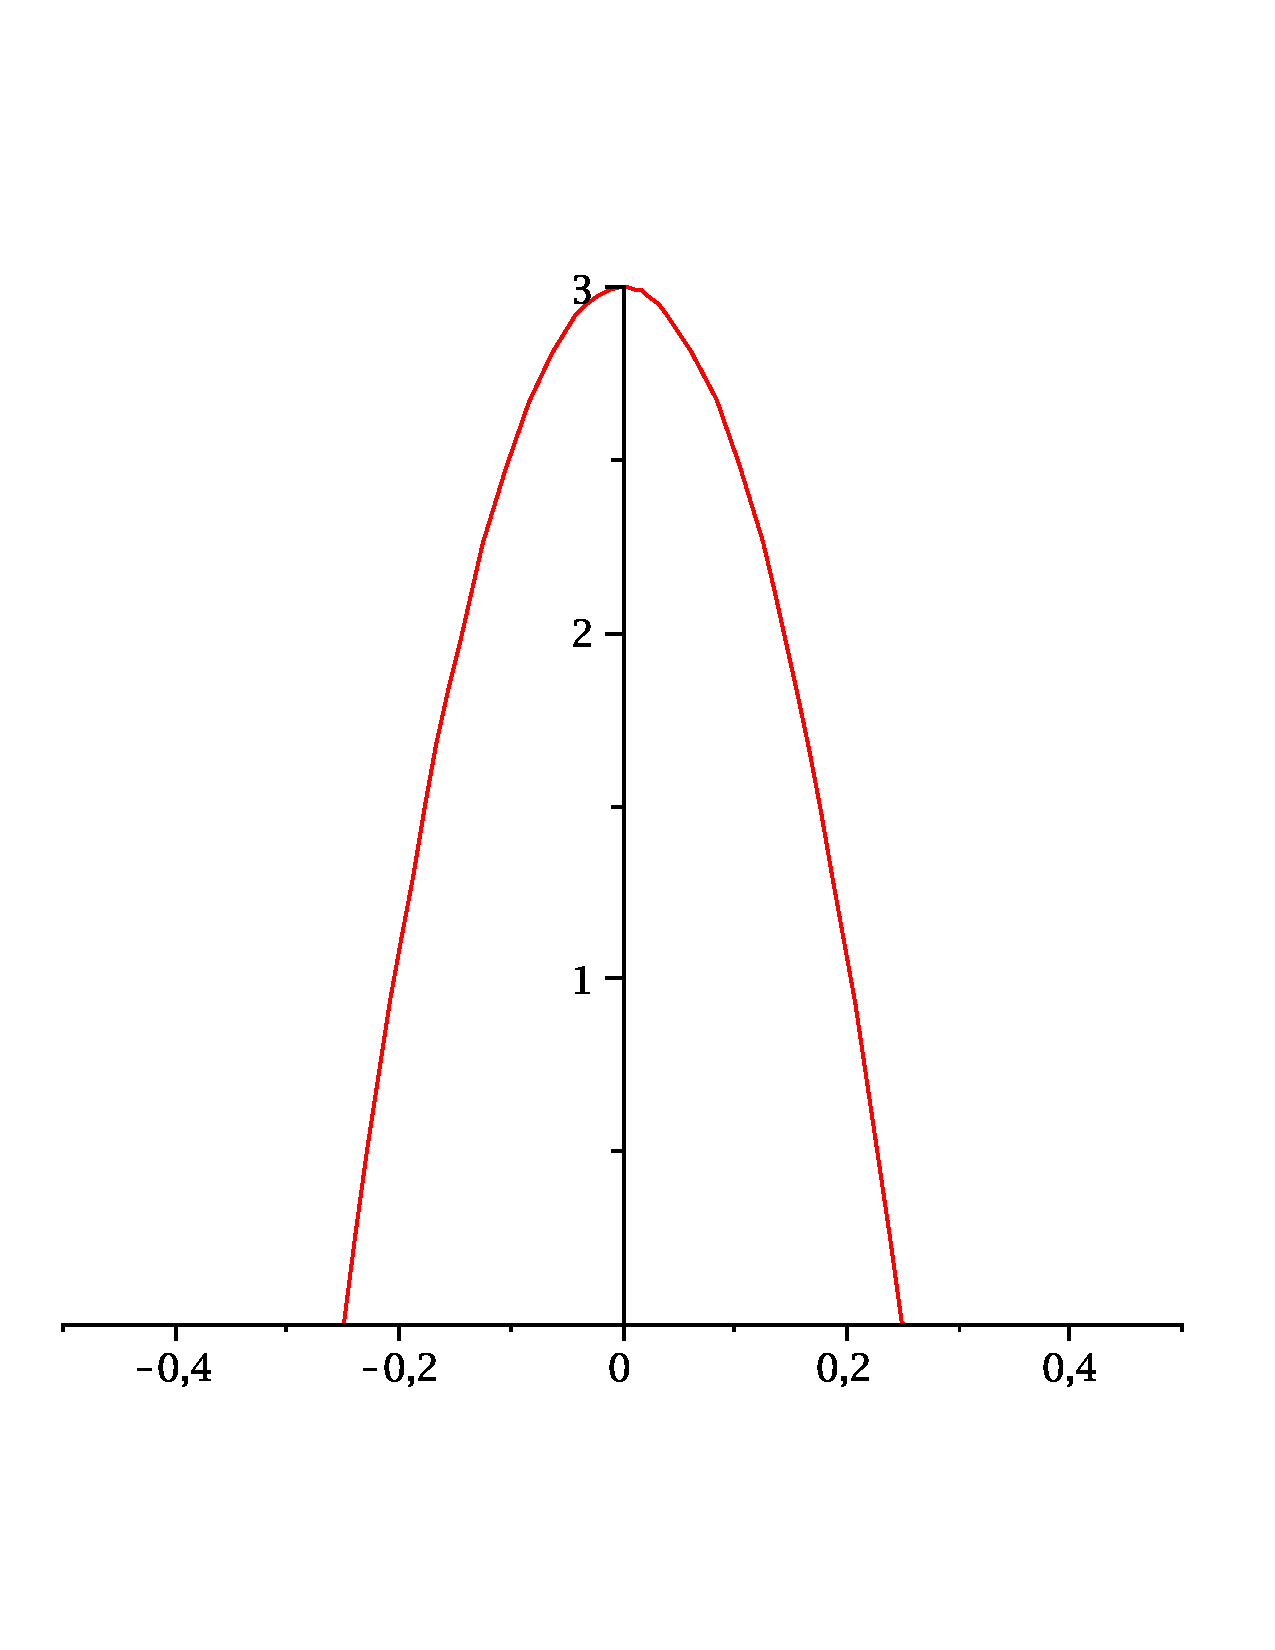
\includegraphics[width=8cm]{Cconv1_1.pdf}
 % Cconv1_1.pdf: 612x792 pixel, 72dpi, 21.59x27.94 cm, bb=0 0 612 792
 \caption{graphe de $\varphi_n$ pour $n=4$}
\end{figure}

\item Le calcul de l'intégrale ne présente pas de difficultés.
\begin{displaymath}
 \int_{-\frac{1}{n}}^{\frac{1}{n}}\varphi_n(t)\,dt = \frac{3n}{4}\left( \frac{2}{n}-\frac{n^22}{3n^3}\right) = 1
\end{displaymath}
\end{enumerate}
\item \begin{enumerate}
 \item En faisant le changement de variable $u=x+t$ dans la définition de $f_n(x)$, on obtient :
\begin{displaymath}
 f_n(x) = \int_{x-\frac{1}{n}}^{x+\frac{1}{n}}\varphi_n(u-x)f(u)du
\end{displaymath}
Développons $\varphi_n(u-x)$ et ordonnons suivant les puissances de $u$ avant d'intégrer en utilisant le linéarité
\begin{multline*}
 f_n(x) =\frac{3n}{4}\left( (1-n^2x^2)\int_{x-\frac{1}{n}}^{x+\frac{1}{n}}f(u)du 
+ 2n^2x \int_{x-\frac{1}{n}}^{x+\frac{1}{n}}uf(u)du \right.\\
\left.-n^2 \int_{x-\frac{1}{n}}^{x+\frac{1}{n}}u^2f(u)du\right)  
\end{multline*}
Les trois intégrales qui figurent dans la parenthèse s'expriment à l'aide de primitives de $u\rightarrow f(u)$, $u\rightarrow uf(u)$, $u\rightarrow u^2f(u)$. Cette expression montre donc bien que $f_n$ est $\mathcal C^1$.
\item  L'expression précédente permet le calcul de $f'_n(x)$.
\begin{multline*}
 f'_n(x)=\frac{3n}{4}\left(
-2n^2x \int_{x-\frac{1}{n}}^{x+\frac{1}{n}}f(u)du\right. \\
\left. +(1-n^2x^2)\left[ f(x+\frac{1}{n})- f(x-\frac{1}{n})\right]\right. \\
\left. +2n^2 \int_{x-\frac{1}{n}}^{x+\frac{1}{n}}uf(u)du \right. \\
\left. +2n^2x\left[ (x+\frac{1}{n})f(x+\frac{1}{n})- (x-\frac{1}{n})f(x-\frac{1}{n})\right]\right. \\
\left. -n^2\left[ (x+\frac{1}{n})^2f(x+\frac{1}{n})- (x-\frac{1}{n})^2f(x-\frac{1}{n})\right]
  \right) 
\end{multline*}
Développons et regroupons les termes en $f(x+\frac{1}{n})$ et $f(x-\frac{1}{n})$. Ils s'annulent et il ne reste que les intégrales qui se regroupent en
\begin{displaymath}
 f'_n(x)=\frac{3n^3}{2}\int_{x-\frac{1}{n}}^{x+\frac{1}{n}}(u-x)f(u)du
\end{displaymath}
Le changement de variable $t=u-x$ dans cette dernière intégrale conduit au résultat demandé:
\begin{displaymath}
 f'_n(x)=\frac{3n^3}{2}\int_{-\frac{1}{n}}^{\frac{1}{n}}tf(x+t)\,dt
\end{displaymath}
\end{enumerate}
\item \begin{enumerate}
 \item Utilisons le calcul de l'intégrale de $\varphi_n$ pour exprimer la différence comme une intégrale que l'on majore de manière très classique :
\begin{multline*}
 |f_n(x)-f(x)|= 
\left\vert 
  \int_{-\frac{1}{n}}^{\frac{1}{n}}\varphi_n(t)f(x+t)\,dt
  - f(x)\int_{-\frac{1}{n}}^{\frac{1}{n}}\varphi_n(t)\,dt
\right\vert \\
= 
\left\vert 
  \int_{-\frac{1}{n}}^{\frac{1}{n}}\varphi_n(t)(f(x+t)-f(x))\,dt
\right\vert
\leq \int_{-\frac{1}{n}}^{\frac{1}{n}}\varphi_n(t)\left\vert f(x+t)-f(x)\right\vert \,dt\\
\leq \int_{-\frac{1}{n}}^{\frac{1}{n}}\varphi_n(t)M_n(x)\,dt 
= M_n(x)\int_{-\frac{1}{n}}^{\frac{1}{n}}\varphi_n(t)\,dt = M_n(x)
\end{multline*}
On a utilisé le fait que $\varphi_n$ est à valeurs positives dans l'intervalle.
\item Dans cette question, on utilise le théorème de Heine. Toute fonction continue sur un segment est \emph{uniformément} continue.\newline
Pour tout $\varepsilon>0$, il existe un $\alpha>0$ tel que , pour tous $x$ et $y$ dans $J$:
\begin{displaymath}
 |x-y|<\alpha \Rightarrow |f(x)-f(y)|<\varepsilon
\end{displaymath}
Considérons un entier $N>\frac{1}{\alpha}$. Alors $n\geq N$ entraine $\frac{1}{n}<\alpha$. 
Pour tout $x$ dans $J$ et $n\geq N$, $M_n(x)<\varepsilon$ donc $K_n(J)<\varepsilon$. Ceci entraine que $\left(K_n(J) \right)_{n\in\N^*}$ converge vers $0$. 
\item Pour tout réel $x$ fixé, on peut considérer un segment $J$ qui le contienne (par exemple de longueur $1$ et de milieu $x$). La question précédente prouve la convergence vers $0$ de la suite des $K_n$ attachée à ce segment.Comme
\begin{displaymath}
 |f_n(x)-f(x)|\leq K_n
\end{displaymath}
On en déduit que $\left(f_n(x) \right)_{n\in\N^*}$ converge vers $f(x)$. 
\end{enumerate}
\item \begin{enumerate}
 \item Introduisons le développement définissant $R_x$ dans l'expression de la dérivée trouvée en 2.b. Par linéarité, on obtient :
\begin{multline*}
 f'_n(x)=\frac{3n^3}{2}f(x)\left( \int_{-\frac{1}{n}}^{\frac{1}{n}}t\,dt \right) 
+\frac{3n^3}{2}f'(x)\left( \int_{-\frac{1}{n}}^{\frac{1}{n}}t^2\,dt\right)  \\
+\frac{3n^3}{2}\int_{-\frac{1}{n}}^{\frac{1}{n}}t^2R_x(t)\,dt
\end{multline*}
 Si on est particulièrement scrupuleux, on peut se poser la question de la continuité de $R_x$ afin de justifier son intégrabilité. Par définition même, $R_x$ est clairement continue sauf en $0$ où elle n'est pas vraiment définie. On peut prolonger $R_x$ par continuité en posant $R_x(0)=0$ car le fait que $R_x$ converge vers $0$ en $0$ est la définition même de la dérivabilité de $f$ en $x$.\newline
Les intégrales de $t$ et de $t^2$ valent respectivement $0$ et $\frac{2n^2}{3}$. On en déduit :
\begin{displaymath}
 f'_n(x) = f'(x) + \frac{3n^3}{2}\int_{-\frac{1}{n}}^{\frac{1}{n}}t^2R_x(t)\,dt
\end{displaymath}
\item Majorons $|f'_n(x)-f'_n(x)|$ en utilisant les expressions précédentes.
\begin{multline*}
 \left\vert f'_n(x)-f'_n(x) \right \vert 
= \frac{3n^3}{2}\left \vert  \int_{-\frac{1}{n}}^{\frac{1}{n}}t^2R_x(t)\,dt \right\vert
\leq \frac{3n^3}{2} \int_{-\frac{1}{n}}^{\frac{1}{n}}t^2\left\vert R_x(t) \right \vert \,dt \\
\leq \frac{3n^3}{2} \int_{-\frac{1}{n}}^{\frac{1}{n}}t^2 \max_{t\in[-\frac{1}{n},\frac{1}{n}]}|R_x(t)| \,dt = \max_{t\in[-\frac{1}{n},\frac{1}{n}]}|R_x(t)|
\end{multline*}
Comme, pour $x$ fixé, $R_x$ converge vers $0$ en $0$, la suite des $\max_{t\in[-\frac{1}{n},\frac{1}{n}]}|R_x(t)|$ converge vers $0$. On en déduit que $\left(f_n'(x) \right)_{n\in\N^*}$ converge vers $f'(x)$.
\end{enumerate}
\end{enumerate}
